\newcommand\user[2]{
	\begin{scope}[xshift=#1cm, yshift=#2cm]
		\clip (0, 0) circle (0.5);
		\fill[black] (0, 0) circle (0.5);
		\fill[white] (0, 0) circle (0.48);
		\fill[black] (0, -0.675) circle (0.4);
		\fill[black] (0, 0.075) circle (0.24);
	\end{scope}
}

\newcommand\ip[2]{
	\begin{scope}[xshift=#1cm, yshift=#2cm]
		%\rectangle[fill=black, rounded corners=0.2cm] (-0.5, -0.7) -- (0.5, 0.7);
		\draw[fill=black, thick, rounded corners=0.15cm] (-0.3, -0.5) rectangle (0.3, 0.5);
		\draw[fill=white] (0, -0.3) circle (0.1);
		\draw[fill=white, rounded corners=0.07cm] (-0.2, -0.1) rectangle (0.2, 0.0);
		\draw[fill=white, rounded corners=0.07cm] (-0.2, 0.1) rectangle (0.2, 0.2);
		\draw[fill=white, rounded corners=0.07cm] (-0.2, 0.3) rectangle (0.2, 0.4);
	\end{scope}
}

\newcommand\www[2]{
	\begin{scope}[xshift=#1cm, yshift=#2cm]
		\clip (0, 0) circle (0.5);
		\fill[yellow!65!black] (0, 0) circle (0.5);
		\fill[white] (-0.5, -0.175) rectangle (0.5,0.175);
		\node[text=yellow!65!black] at (0,0) {www};
	\end{scope}
}

\newcommand\malwww[2]{
	\begin{scope}[xshift=#1cm, yshift=#2cm]
		\clip (0, 0) circle (0.5);
		\fill[red!65!black] (0, 0) circle (0.5);
		\fill[white] (-0.5, -0.175) rectangle (0.5,0.175);
		\node[text=yellow!65!black] at (0,0) {www};
	\end{scope}
}

\newcommand\wwwline[3]{
	\node[circle, minimum size=1.1cm] (#3) at (0, #1) {};
	\www{0}{#1}
	\node[text width=50mm, align=right] at (-5, #1) {#2};
}

\newcommand\malwwwline[3]{
	\node[circle, minimum size=1.1cm] (#3) at (0, #1) {};
	\malwww{0}{#1}
	\node[text width=50mm, align=right] at (-5, #1) {#2};
}

\newcommand\userline[2]{
	\node[circle, minimum size=1.1cm] (#2) at (5, #1) {};
	\user{5}{#1}
	\node[text width=50mm, align=left] at (10, #1) {#2};
}

\newcommand\ipline[3]{
	\node[circle, minimum size=1.1cm] (#3) at (5, #1) {};
	\ip{5}{#1}
	\node[text width=50mm, align=left] at (10, #1) {#2};
}


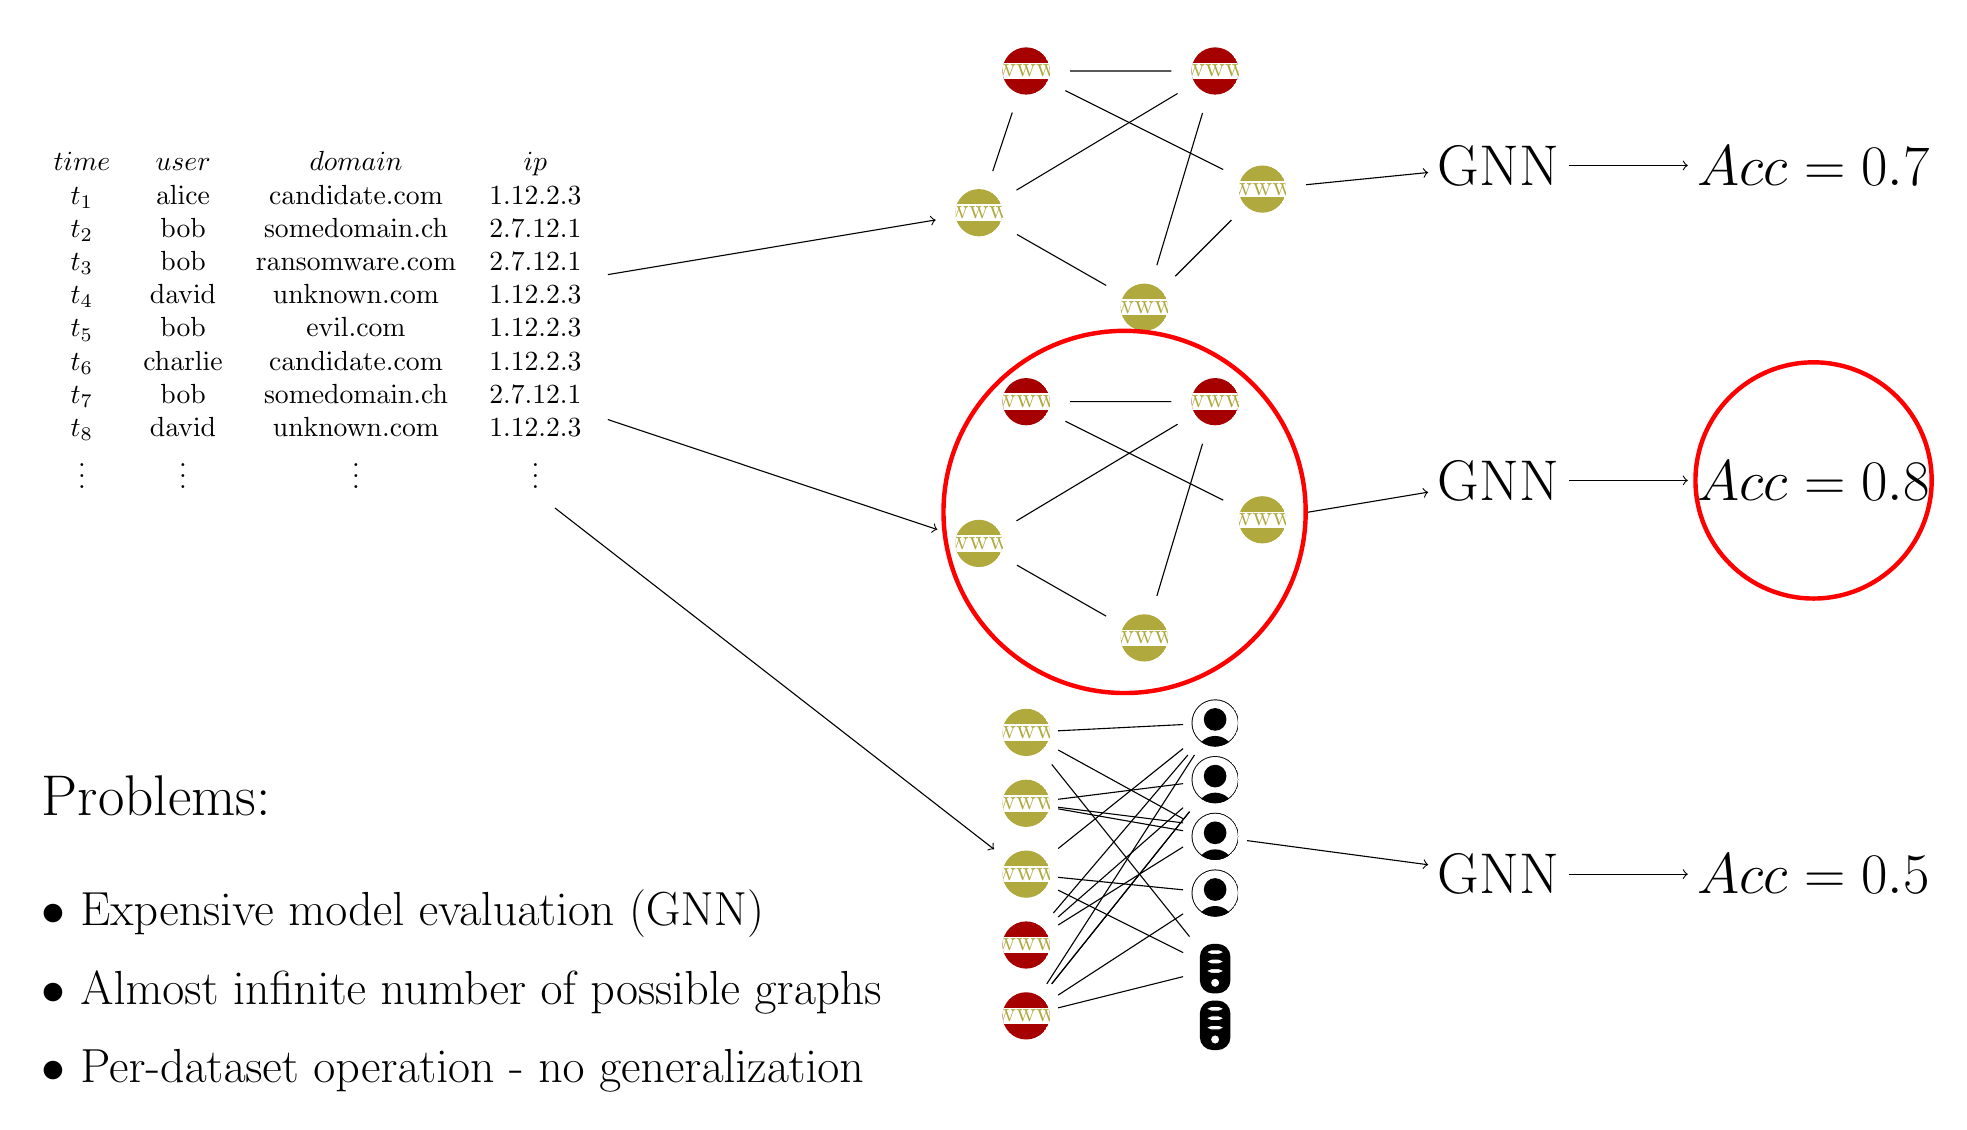
\begin{tikzpicture}

\node at (-15, 4) (x)
{
\begin{tabular}{cccc}
    \toprule
    $\bm{time}$ & $\bm{user}$ & $\bm{domain}$ & $\bm{ip}$ \\
    \midrule
    $t_1$&alice& candidate.com& 1.12.2.3\\
    $t_2$&bob& somedomain.ch& 2.7.12.1\\
    $t_3$&bob& ransomware.com& 2.7.12.1\\
    $t_4$&david& unknown.com & 1.12.2.3\\
    $t_5$&bob& evil.com & 1.12.2.3 \\
    $t_6$&charlie& candidate.com & 1.12.2.3 \\
    $t_7$&bob & somedomain.ch& 2.7.12.1 \\
    $t_8$&david& unknown.com & 1.12.2.3\\
    \vdots &\vdots &\vdots &\vdots \\
    \bottomrule
\end{tabular}
};

\begin{scope}[scale=0.6, xshift=-8cm, yshift=9cm]  
\node[circle, minimum size=1.1cm] (d1) at (-2, 3) {};
\malwww{-2}{3}	
\node[circle, minimum size=1.1cm] (d2) at (2, 3) {};
\malwww{2}{3}	
\node[circle, minimum size=1.1cm] (d3) at (-3, 0) {};
\www{-3}{0}
\node[circle, minimum size=1.1cm] (d4) at (3, 0.5) {};
\www{3}{0.5}	
\node[circle, minimum size=1.1cm] (d5) at (0.5, -2) {};
\www{0.5}{-2}
\draw (d1) -- (d2);
\draw (d1) -- (d3);
\draw (d1) -- (d4);
\draw (d2) -- (d3);
\draw (d2) -- (d5);
\draw (d3) -- (d5);
\draw (d4) -- (d5);
\end{scope}

\begin{scope}[scale=0.6, xshift=-8cm, yshift=2cm]  
\node[circle, minimum size=1.1cm] (d11) at (-2, 3) {};
\malwww{-2}{3}	
\node[circle, minimum size=1.1cm] (d22) at (2, 3) {};
\malwww{2}{3}	
\node[circle, minimum size=1.1cm] (d33) at (-3, 0) {};
\www{-3}{0}
\node[circle, minimum size=1.1cm] (d44) at (3, 0.5) {};
\www{3}{0.5}	
\node[circle, minimum size=1.1cm] (d55) at (0.5, -2) {};
\www{0.5}{-2}
\draw (d11) -- (d22);
\draw (d11) -- (d44);
\draw (d22) -- (d33);
\draw (d22) -- (d55);
\draw (d33) -- (d55);
\end{scope}

\begin{scope}[scale=0.6,  xshift=-8cm, yshift=-6cm]   
  \malwww{-2}{-2} \node[minimum size=0.8cm] at (-2, -2) (D1) {};
  \malwww{-2}{-0.5}  \node[minimum size=0.8cm] at (-2, -0.5) (D2) {};
  \www{-2}{4} \node[minimum size=0.8cm] at (-2, 4) (D5) {};
  \ip{2}{-1} \node[minimum size=0.8cm] at (2, -1) (i1) {};
  \user{2}{4.2} \node[minimum size=0.8cm] at (2, 4.2)(Alice) {};
  \draw (Alice) -- (D1);
  \draw (Alice) -- (D2);
  \draw (i1) -- (D1);
  \draw (Alice) -- (D5);
  \draw (i1) -- (D5);
  \www{-2}{1}  \node[minimum size=0.8cm] at (-2, 1) (D3) {};
  \www{-2}{2.5}  \node[minimum size=0.8cm] at (-2, 2.5) (D4) {};
  \ip{2}{-2.2}  \node[minimum size=0.8cm] at (2, 2) (i2) {};
  \user{2}{0.6}  \node[minimum size=0.8cm] at (2, 0.6) (David) {};
  \user{2}{1.8}  \node[minimum size=0.8cm] at (2, 1.8) (Charlie) {};
  \user{2}{3}  \node[minimum size=0.8cm] at (2, 3) (Bob) {};
  \draw (Alice) -- (D3);
  \draw (Bob) -- (D1);
  \draw (Bob) -- (D2);
  \draw (Bob) -- (D1);
  \draw (David) -- (D1);
  \draw (i2) -- (D2);
  \draw (Bob) -- (D4);
  \draw (David) -- (D3);
  \draw (Charlie) -- (D4);
  \draw (Charlie) -- (D5);
  \draw (i1) -- (D3);
  \draw (i2) -- (D4);

\end{scope}

%\node[font=\huge] (g0) at (-4, 6) {$\mathcal{G}_0$};
%\node[font=\huge] (g1) at (-4, 5) {$\mathcal{G}_1$};
%\node[font=\huge] (gn) at (-4, 2) {$\mathcal{G}_N$};

\draw[->] (x)--(d3);
\draw[->] (x)--(D3);
\draw[->] (x)--(d33);

\node[font=\huge] (m0) at (0, 6) {GNN};
\node[font=\huge] (m1) at (0, 2) {GNN};
\node[font=\huge] (mn) at (0, -3) {GNN};

\draw[->] (d4)--(m0);
\draw[->] (d44)--(m1);
\draw[->] (Charlie)--(mn);

\node[font=\huge] (p0) at (4, 6) {$Acc=0.7$};
\node[font=\huge] (p1) at (4, 2) {$Acc=0.8$};
\node[font=\huge] (pn) at (4, -3) {$Acc=0.5$};

\draw[->] (m0)--(p0);
\draw[->] (m1)--(p1);
\draw[->] (mn)--(pn);



\uncover<2-3>{
  \draw[color=red, ultra thick] (4, 2) circle (1.5cm);
}

\uncover<3>{
  \draw[color=red, ultra thick] (-4.75, 1.6) circle (2.3cm);
}

\uncover<3->{
    \node[font=\huge, text width=110mm, align=left] at (-13, -2) {
{Problems:}
};
    \node [font=\LARGE, text width=110mm, align=left] (top)    at (-13,-3.5) {$\bullet$ Expensive model evaluation (GNN)};
    \node [font=\LARGE, text width=110mm, align=left] (middle) at (-13,-4.5)
    {$\bullet$ Almost infinite number of possible graphs};
    \node [font=\LARGE, text width=110mm, align=left] (bottom) at (-13,-5.5)  {$\bullet$ Per-dataset operation - no generalization};
}
\end{tikzpicture}
